\documentclass{article}
\usepackage[utf8]{inputenc}
\usepackage{authblk}
\usepackage{xcolor}
% for arrows and other symbols
\usepackage{textcomp}

\title{//TODO ein Titel}
\author[1]{Alexander Bigga, Martin Brändle, Ronny Bölter, Constanze	Decker, Maria España, Gerhard Eilbacher, Matthias Flasko, Frank Krabbes, August H. Leugers-Scherzberg, Marianna Mühlhölzer, Dennis	Müller, Philip	Münch, Tom	Niers, Daniel Nüst, Adrian	Pachzelt,  Maximilian Plich, Ronald	Steffen, Klaus 	Thoden, Hanna Varachkina, Paul Warner, Nils Weiher, Daniela	Wolf, Dulip	Withanage}

 
\date{20-21. February 2020}

\usepackage{natbib}
\usepackage{graphicx}
\usepackage{hyperref}
\begin{document}

\maketitle

\begin{abstract}
    //TODO 
\end{abstract}
\tableofcontents
\newpage


\section{Import/Export-Plugin}
\author{Philip Münch, Alexander Bigga, Mariana España}

\subsection{Current Situation}

\begin{itemize}
    \item Native XML plugin can only export/import issues/articles, and only metadata and galley files, not workflow uploads, messages or user accounts.
    \item There is a user account import/export plugin.
    \item There is no way to import/export journal settings.
    \item Import/Export plugins are callable from the command line, so that automatic backups can be done this way.
   \item The new REST API provides lists of journals, issues and articles
\end{itemize}

\subsection{Open Issues}

\begin{itemize}
\item 19.02.2020 (!) “option to reference files in export xml” (\url{https://github.com/pkp/pkp-lib/pull/5524})
\begin{itemize}
\item On export the files can be excluded from embedding in XML. The files are referenced by href instead.
\end{itemize} 
\item 11.01.2018: Extend native import/export plugin to include additional entities (\url{https://github.com/pkp/pkp-lib/issues/3261})
\begin{itemize}
\item Open PRs: OJS (\url{https://github.com/pkp/ojs/pull/1978}), PKP-Lib (\url{https://github.com/pkp/pkp-lib/pull/3722})
\item For OJS 2.x there has been an \url{https://github.com/lepidus/fullJournalTransfer}) plugin.
\end{itemize} 
\item \url{https://github.com/pkp/pkp-lib/issues/5067} (OJS2 -> OJS3 via XML exports)
\item \url{https://github.com/pkp/pkp-lib/issues/4880} (native XML plugin needs to be changed to support versioning)
\end{itemize} 

\subsection[{Use cases}]{\label{n9obwgh5nm6w}Use cases}
\begin{itemize}
\item Migrating between instances 
\begin{itemize}
\item Preparatory and productive instance
\item Migrating a journal to a different service provider
\end{itemize} 
\item Backing up journals independently on multi-journal instances
\end{itemize} 

\subsection[{Goal}]{\label{e4lpz19m7e47}Goal}
\begin{itemize}
\item We need a way to export a full journal. 
\item The task could be divided into multiple steps:
\begin{itemize}
\item Exporting journal settings (There is no way to do this at present)
\item Exporting users(This can already be done)
\item Exporting all issues (The Native XML Plugin already does part of this)
\end{itemize} 
\item Since the size of a single export file in XML format with Base64-encoded files would be impractical for a full journal, this seems like the best solution.
\end{itemize} 
\subsection[{What needs to be done}]{\label{56w7y5hscs4v}What needs to be done}
\begin{itemize}
\item The Native XML plugin needs to be extended to also export all interry workflow files and all messages (optionally).
\item A new plugin has to be created to export journal settings. This should be callable from the command line as well for automatic backup purposes.
\end{itemize} 
\subsection[{Problems we see}]{\label{vfybgm5yfkwb}Problems we see}\par
If all workflow results are to be imported again, there needs to be a way to link them back to the users that produced them. What happens if a user is not present? \par
We propose to separate between “people” records that are created per journal, and account records that are global. These can be linked and unlinked. We suspect this might also be a good idea for GDPR compliance.
\subsection[{Results}]{\label{c4kqlfgcopb9}Results}\par
We decided to just ask for a current status on the main issue above, since some work has already been done that would fulfill our needs, but we are not able to discern how far this has come.\par
Regarding implementing a new plugin for importing/exporting journal settings, we will need more information on how such a plugin would be implemented and what provisions might already be in the code.\par
 
\section{Suche (Elastic-Search / Solr / Lucene)}

\author{Nils Weiher, Constanze Decker, Tom Niers}


\subsection[{Current Situation}]{\label{4aeirk1scnvf}Current Situation}

\begin{itemize}
\item Zur Zeit nur ein Plugin für die Suche mit Solr: “Lucene Plugin”

\begin{itemize}
\item \url{https://github.com/ojsde/lucene/}
\item Entwickelt von CEDIS, FU Berlin
\item Bald in OJS Plugin Gallery (laut Ronald Steffen) 
\end{itemize} 
\item Ein Artikel zum Vergleich von Solr und ElasticSearch: \url{https://logz.io/blog/solr-vs-elasticsearch/}
\end{itemize} 
\subsection[{Goal}]{\label{309dd9qucqop}Goal}
\begin{itemize}
\item Vergleich ElasticSearch und Solr
\item Analyse vom aktuellen Stand lucene Plugin
\item Klären ob weg über SuchPlugin oder API?
\end{itemize} 
\subsection[{Results}]{\label{6b7urgumedb2}Results}
\begin{itemize}
\item Für Instanz übergreifende Suche und Suche in OMP und OJS zusammen, gibt es anscheinend noch keine bestehende Lösung. In UB Heidelberg wird eine eigene Lösung mit Hilfe von Solr entwickelt zur suche in allen online Publikationen.
\item Nach Diskussionen und Austausch sind wir auf Plugin Entwicklung im Allgemeinen umgestiegen
\item Das bestehende Plugin auf ElasticSearch umzuschreiben, wäre möglich aber mit viel Aufwand verbunden, da die Konfiguration und das Schema speziell für Solr entwickelt ist und auch die bestehende Methoden XML Erzeugen für die Weitergabe an Solr.{\hskip1pt}\\{}Für ElasticSearch müsste das in eine JSON Struktur umgeschrieben werden und die ElasticSearch Konfiguration müsste man auch von vorne anfangen.
\end{itemize} 
\section{Plugin for connecting external Long-term archiving systems (Rosetta, Archivematica, Dataverse, DSpace/Sword, …)}

\author{Gerhard Eilbacher, Ronny Bölter, Martin Brändle, Paul Warner}

\subsection[{Goal}]{\label{13mtyhwidjmu}Goal}

\begin{itemize}
\item Generic Plugin (Able to connect with different systems) 
\item Plugin enables User to choose which files to send from OJS to long-term Archives
\item Plugin features functionality to validate file formats, integrity of content and if all required Metadata has been provided
\end{itemize} 
\subsection[{Questions to be answered}]{\label{78nkvdvvmi5r}Questions to be answered}
\begin{itemize}
\item What must be archived on article level? Possibilities:
\begin{itemize}
\item Only metadata and published galleys/supplements
\item Metadata, published galleys/supplements including all versions (OJS 3.2!)
\item All above, including reviewer reports
\item All above, including article history
\end{itemize} 
\end{itemize} \par
These options should be configurable by journal manager{\hskip1pt}\\{}Think of long-term archiving as >10 years; with a digital archive it should be possible to reconstruct the history or development of an article/issue/journal
\begin{itemize}
\item Who can archive?
\begin{itemize}
\item Journal manager
\item Special role within OJS?
\item Should not be given to roles such as author, reviewer, editor
\end{itemize} 
\end{itemize} 
\begin{itemize}
\item Packaging : What is in an archival package?
\begin{itemize}
\item Individual article
\item Selected articles
\item Only published articles / all articles?
\item A complete issue
\item A complete journal
\end{itemize} 
\end{itemize} 
\begin{itemize}
\item What must be delivered?
\begin{itemize}
\item Some archival software require either complete archival packages (e.g. Submission Information Package (SIP) including METS archival format description), others just individual metadata and files to be archived. In the latter case, the data stewart of the digital archive will create the package.
\end{itemize} 
\item Push or pull mechanism? (we prefer push)
\begin{itemize}
\item Push: OJS delivers a package to archive
\item Pull or harvesting (oai): OJS prepares a download section with a archival “package”, digital archive fetches it (e.g. manually or automatically). Disadvantages: Who is allowed to pull? 
\end{itemize} 
\end{itemize} 
\subsection[{Requirements}]{\label{w7kwrjjhkztc}Requirements}


\begin{figure}[h!]
\centering
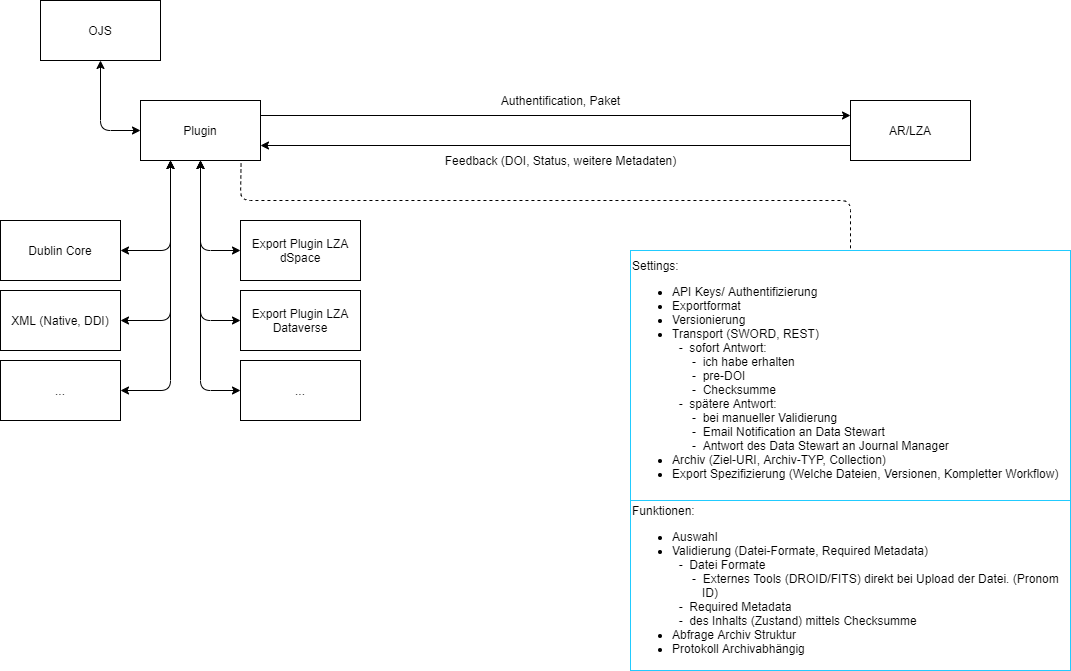
\includegraphics[scale=0.3]{resource1.png}
\caption{}
\label{fig:universe}
\end{figure}

\subsection[{Workflow}]{\label{qt8vsct0yswp}Workflow}
\begin{itemize}
\item The archival plugin must hook in at various points of the OJS workflow
\begin{itemize}
\item Upload of files: Fixity (e.g. MD5 checksum) check, file format identification
\item Delivery of archival “package” (again fixity check should be made before)
\end{itemize} 
\item Delivery of package: Depending on digital archive and its configuration, there may be a non-interactive or a interactive workflows:
\begin{itemize}
\item Non-interactive: Archive accepts package, validates it, and if valid puts it into archival storage without human interaction. A delivery receipt including acceptance status is sent back. Interaction is continuous, but may be async. Example for such archive softwares may be repositories such as DSpace or EPrints, or DLCM
\item Interactive: Package goes to a pre-ingest or ingest buffer, where it is validated by a data steward, and if valid, packaged (e.g. according to OAIS standards). Data steward sends back delivery receipt including acceptance status (e.g. archived, rejected). Communication is completely async, and there may be days or weeks between messages. Example for such archive softwares may be Archivematica or DLCM
\end{itemize} 
\item Upon delivery of a “package”, plugin sends a notification message (e.g.) to the data steward of the archive
\end{itemize} \par
{\itshape Dataflow}\par
{\itshape Modular setup}
\begin{itemize}
\item Plugin communicates with OJS plugin for archival software (via pipe / internal API)
\item OJS archival software plugins (DSpace, …) communicate with export format plugins for metadata format creation (e.g. DC, DataCite XML Schema, METS, …)
\item Plugin has specified communication protocol with archival software (e.g. Sword/REST, …)
\item Plugin may send metadata and files in a “loose” package or may send everything in a compressed SIP (e.g. using METS/PREMIS for metadata and format description and files)
\end{itemize} \par
{\itshape GUI}
\begin{itemize}
\item Settings
\item File list: Provides both selection option and status (formats, metadata inputfield, error messages)
\item Button for “package” delivery
\end{itemize} \par
{\itshape Maintenance of the Plugin}
\begin{itemize}
\item Sub-Plugins (for export) have to be kept up-to-date for new versions of archive software and backwards compatible
\item General maintenance (e.g. in case of api changes in sub-plugins)
\end{itemize} \par
{\itshape Datastructure}
\begin{itemize}
\item Metadata of the article should be enhanced with
\begin{itemize}
\item Status in workflow: Not archived, in review, archived, …
\item Checksums (for metadata, for each file) for fixity checks
\item File format identifier (e.g. PRONOM fmt)
\end{itemize} 
\item Plugin should have an internal list of valid file formats (e.g. a list of PRONOM format identifiers) for long term archiving (e.g. various PDF/A formats, text formats such as JSON, CSV, etc.)
\item Plugin should have a knowledge about mandatory metadata for each archive software configured
\end{itemize} 

 


\section{Docker\-basierte Entwicklungsumgebungen und Automatisierung}

\author{Daniel Nüst, Dennis Müller, Dulip Withanage}

\subsection{Goal}
{\bfseries Eine einfache Schritt-für-Schritt Anleitung zu einer Entwicklungsumgebung, mit der man OJS Plug-ins entwickeln kann. Die Anleitung enthält auch die Schritte um mit üblichen IDEs eine Debugging-Session zu starten.}\par
Dies ist insbesondere für Gelegenheits-Entwickler hilfreich. Der Ansatz liefert eine Alternative für git submodules für Plug-ins bzw. Klonen des Plug-in-Projektes direkt in den Plug-in-Ordner.\par
Die Laufzeitumgebung sollte lokal so gekapselt sein, dass der OJS Quellcode auf dem Entwicklerrechner in einen Container gemountet und dann OJS (in bestimmter Version) gestartet werden kann. Mit einem Klick kann der Entwickler aus seiner Wunsch-IDE debuggen:
\begin{itemize}
\item VSCode
\item Atom
\item …
\end{itemize} 
User workflow:


\begin{enumerate}
\item {\itshape docker run --rm -it --volume \$(pwd)/my-ojs-plugin:/var/ojs/.../plugins:ro -p 8081:8081 -p 9000:9000 ojs-dev:3.1.2}
\item Debugging in IDE starten
\item Beim Bearbeiten von Templates innerhalb eines Plug-ins: ggf noch Frontend-Cache löschen
\end{enumerate}
\subsection[{Aufgaben}]{\label{2nr34glqlyi}Aufgaben}
\begin{enumerate}
\item Offizielle Docker images ausprobieren
\item Abgeleiteten Dockerfile schreiben mit Entwicklungseinstellungen
\begin{enumerate}
\item Xdebug
\item Ports
\item Gemountete (plugin-)directories (s. “Volumes” in docker-compose.yml)
\end{enumerate}
\item Workflow auf den Rechnern alle Gruppenmitglieder testen
\item Anleitung zur Nutzung des Entwicklungs-Dockerfiles
\item PR öffnen an \url{https://www.github.com/pkp/docker-ojs}
\end{enumerate}
\subsection[{Results}]{\label{ijros8fzbxm}Results}
\begin{itemize}
\item Sichtung \url{https://www.github.com/pkp/docker-ojs} und der docker-compose Konfigurationen

\begin{itemize}
\item \url{https://github.com/pkp/docker-ojs/issues/12}
\end{itemize} 
\item Telefonat mit Marc > neues Änderungen gepusht, Hintergründe erläutert
\item Funktionierendes Image: 3.1.2-4 mit Apache und PHP7 
\begin{itemize}
\item localMake.sh
\item docker-compose up
\item Im browser: \url{http://localhost:8081/index/install}
\item Database settings: ojs, ojs, ojs
\end{itemize} 
\item Dennis kann jetzt Docker
\item Daniel hat einen PR geöffnet mit einem Vorschlag für eine alternative Handhabung der compose Konfigurationen und einer aktualisierten README: \url{https://github.com/pkp/docker-ojs/pull/14}
\end{itemize} 
 
\section{XML-Workflow}

\author{Adrian Pachzelt, Klaus Thoden, Marianna Mühlhölzer, Hanna Varachkina, Ronald Steffen, Matthias Flasko, August H. Leugers-Scherzberg, Maximilian Plich}
\subsection[{Goal}]{\label{e5qdlbvq435o}Goal}
\begin{itemize}
\item Mögliche Workflows von Office-Formaten (docx) über XML (TEI-P5) zu verschiedenen Ausgabeformaten (HTML, PDF, JATS, EPUB, …) ausarbeiten
\item Workflows sollen individuell konfiguriert werden können
\item Workflow soll innerhalb von OJS verwendbar sein
\end{itemize} 
\subsection[{Ressources}]{\label{wu30zlf94kvp}Ressources}
Overview of XML import tools dedicated to PKP uses (from 2018 sprint): \url{https://docs.google.com/spreadsheets/d/1XiLtorlsLHFJZzbkBNRcSnQav80yODyV9z1oKE74Tyo/edit\#gid=0}
\subsection{Front-end Gruppe}
\begin{enumerate}
\item Eingabe-Format wählen (vlt. Dropdown Menu): docx, odt, etc.
\item Metadaten
\item Zitate (regular expressions)
\item Bilder
\item Ausgabe-Format wählen: HTML, Jats, etc. 
\end{enumerate}
\subsection[{Results}]{\label{mvi15gtcieym}Results}
\subsubsection{docx-Konvertierung mit Kommandozeile-Konverter}
\begin{enumerate}
\item Tools
\begin{enumerate}
\item myTypeset (Fußnoten müssen separat gesetzt werden)
\item docxConverter (keine Fußnoten, Zitate nur mit Nummerierungen)
\item Pandoc native
\item oxGarage
\end{enumerate}
\item Anforderungen
\begin{enumerate}
\item Autoren müssen sich an definierte Dokument-Templates und redaktionelle Vorgaben halten
\item Feste Parameter für die Konvertierung müssen konfiguriert werden können (auf welcher Ebene? Hosting, Journal Manager/Editor)
\item Variable Parameter müssen abgefragt werden
\item Referenzen müssen standardisiert werden, parsing muss extra implementiert werden
\item Automatisiertes post-processing müss möglich sein
\item Manuelle Nachbearbeitung wird immer nötig sein
\item Individuelle zusätzlich Bearbeitungsschritte müssen integriert werden können z.B. für:
\begin{enumerate}
\item Sprachidentifikation (mit z.B. Tikka) muss integriert werden (für Layout/Silbentrennung), eventuell inklusive Wörterbücher (die gepflegt werden müssen)
\item Anpassung von Lizenzrechten
\end{enumerate}
\item Bearbeitungsverlauf zwischenspeichern und verfügbar machen
\end{enumerate}
\end{enumerate}

\subsubsection{Wunschvorstellung OJS-XML-Editor}
\begin{enumerate}
\item Entwicklung kostet viel Zeit und Geld/Personal
\begin{enumerate}
\item Institutsübergreifendes Projekt?
\item Kommunikation an die Institute
\item Ist Texture eine Möglichkeit? \textrightarrow\ Stand des Plugins? 
\end{enumerate}
\item Backend für Editoren
\item Frontend für Autoren (zum Schreiben und für Revision)
\begin{enumerate}
\item arbeiten direkt in einem OJS-XML-Editor
\item Erfahrungen von vergleichbaren Editoren: Autoren arbeiten in Word und kopieren formatierte Daten
\end{enumerate}
\end{enumerate}
\begin{figure}[htbp]
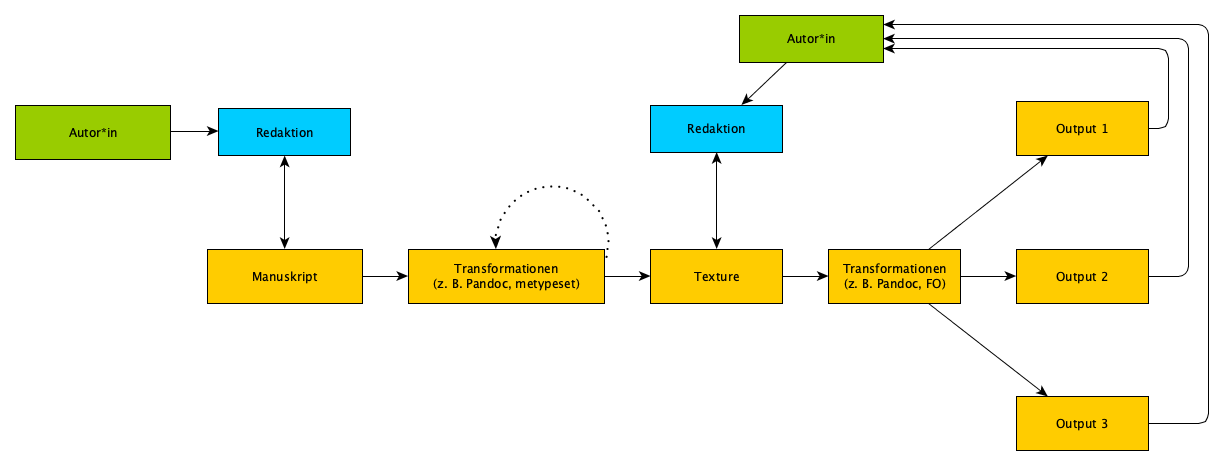
\includegraphics[width=\textwidth]{resource2.png}
\end{figure}

\subsubsection{Praxis}
\begin{itemize}
\item Pandoc, meTypeset, XSLT und Texture verarbeiten nicht immer alle nach JATS erlaubten Tags. Es muss eine Liste von Tag erstellt werden die nicht verwendet werden dürfen.
\item Eine Überprüfung auf Elemente dieser Art muss vor starten der Pipeline erfolgen
\item Informationen übergreifend sammeln (Community-Forum?, ojs-de.net?) und aktualisieren (z.B. bei neuen Versionen) 
\end{itemize}

Beispielkonvertierungen:
\begin{itemize}
\item Pandoc:\par
\verb+pandoc -f docx -t jats --standalone -o <out_file>.xml <in_file>.docx+
\begin{itemize}
\item Ergebnis mit komplexen docx-Dateien (Tabellen + Formeln, nur Formeln): das generierte JATS kann in Texture nicht angezeigt werden: 
\begin{itemize}
\item \verb+<table>+ is not valid
\item \verb+<email>+ not valid (e-mail-Link in Word)
\item einfache Auflistung i), ii), iii) funktioniert nicht
\item Einfache Grafik (ohne Caption) funktioniert nicht
\item \verb+<alternatives>+-Tag in \verb+<inline-formula>+ funktioniert nicht
\item … und viele andere Fehler
\item Nach Entfernung aller Tabellen, Bilder, Formel und Aufzählungen:
\begin{itemize}
\item Keine kommentierte Texture-Fehlermeldung mehr
\item Browser meldet: “ERROR:Node already exists“
\end{itemize} 
\item Gesamte Citavi-Bibliographie wird in einen \verb+<p>+-Tag gepackt
\end{itemize} 

\end{itemize} 
\item myTypeset
\begin{itemize}
\item Keine Konvertierung ohne LibreOffice oder Word auf dem System
\item Hier müsste evtl. in Zusammenarbeit mit dem Entwickler der ReferenceLinker verbessert werden. Vor allem die Erkennung der Referenzliste selber ist noch sehr fehleranfällig.
\end{itemize} 
\item oxGarage:
\begin{itemize}
\item Repositorium: \url{https://github.com/TEIC/Stylesheets}
\end{itemize} 
\end{itemize} \par
Erzeugt mit:\par
\verb+/home/user/dev/Stylesheets/bin/docxtotei --localsource=/home/user/dev/dependencies/TEI EVA\textunderscore Paper\textunderscore b.docx ep\textunderscore b-tei.xml+\par
\verb+/home/user/dev/Stylesheets/bin/teitonlm --localsource=/home/user/dev/dependencies/TEI ep\textunderscore b-tei.xml ep\textunderscore b-jats.xml+
\begin{itemize}
\item Ergebnis: JATS nicht in Texture nicht lesbar: \verb+<caption>+ is not allowed at the current position
\end{itemize} \par
Weiteres Vorgehen:
\begin{itemize}
\item \url{https://github.com/GrazingScientist/OJS-XML-Pipeline-Plugin/tree/master} enthält Beispieldateien
\item Informationsaustausch und Weiterentwicklung über Github-Issues 
\end{itemize} 


%\bibliographystyle{plain}
%\bibliography{references}
\end{document}

